\title{03 Real Series}
\date{Autumn 2019}
\author{Ryan Greenup}
\documentclass[class=article, crop=false]{standalone}
\usepackage{./resources/style}
\begin{document}
\tableofcontents

(03) Series

Wk 4 Material; Topic 3; Due 28 March


\hypertarget{header-n3124}{%
\subsection{The Cauchy Criterion (3.5)}\label{header-n3124}}

\hypertarget{header-n3125}{%
\subsubsection{The Cauchy Convergence Criterion}\label{header-n3125}}

A sequence is convergent if and only if it is a Cauchy sequence

\begin{itemize}
\item
  \textbf{Cauchy Sequence} implies \textbf{Convergence}

  \begin{itemize}
  \item
    Every Cauchy sequence of real numbers is bounded, hence by the
    Bolzano-Weierstrass theorem the sequence has a convergent
    subsequence, hence is itself convergent.
  \end{itemize}
\item
  \textbf{Convergence} imples \textbf{Cauchy Sequence}

  \begin{itemize}
  \item
    If two terms can be made arbitrarily close then any term can be made
    arbitrarily close to another term in the set (which will be the
    limit point).
  \end{itemize}
\end{itemize}

\hypertarget{header-n3138}{%
\subsection{Properly Divergent}\label{header-n3138}}

A series \((x_n)\) is said to be properly divergent if
\(\lim_{n\rightarrow \infty}(x_n) = \pm \infty\)

\hypertarget{header-n3140}{%
	\newpage
\subsection{Definition of a Series {[}3.7.1{]}}\label{header-n3140}}

if \(x_n\) is a sequence, then the \textbf{series} generated by the
sequence is \(S = (s_k)\):

\begin{itemize}
\item
  The terms of the sequence are
  \(x_n) = (x_1, x_2, x_3, x_4, \dots s_n)\)
\end{itemize}

The terms of the series are \((s_n) = (s_1, s_2, s_3, s_4, \dots s_n)\)

The terms of the series are called the \textbf{partial sums} and are
defined as such:

\begin{figure}%[width=7cm]
\centering
\caption[Handwritten Series from Sequence]{Creating a Series from a Sequence}
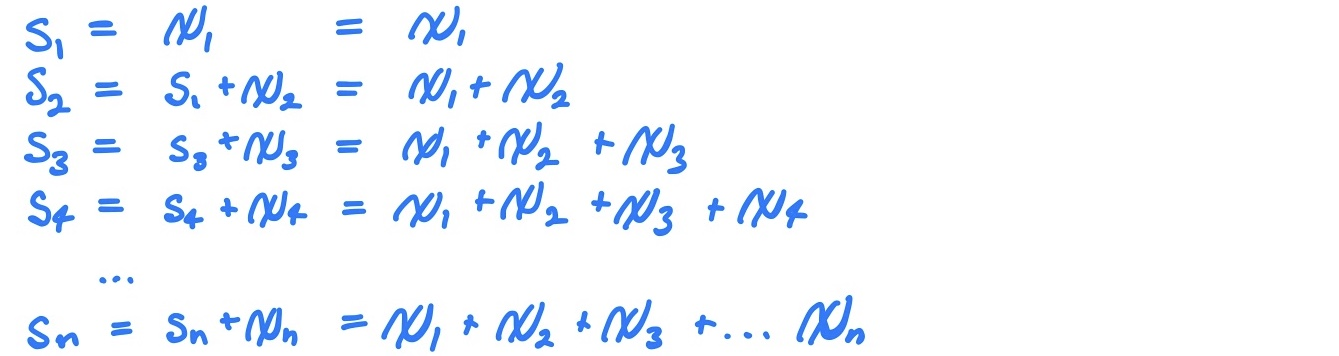
\includegraphics[width=5cm]{media/InfSeries/kdskfdsakj.jpeg}
\end{figure}

\hypertarget{header-n3150}{%
	%\newpage
\subsection{Common Series Types}\label{header-n3150}}

These are series that we are expected to memorise because they so often
appear in series problems (and moreover we we will need them for the
exam).

\hypertarget{header-n3152}{%
\subsubsection{Geometric Series (3.7.6 (a))}\label{header-n3152}}

The Geometric Series is Convergent if and only if \(\mid r \mid < \) :

\begin{figure}
\centering
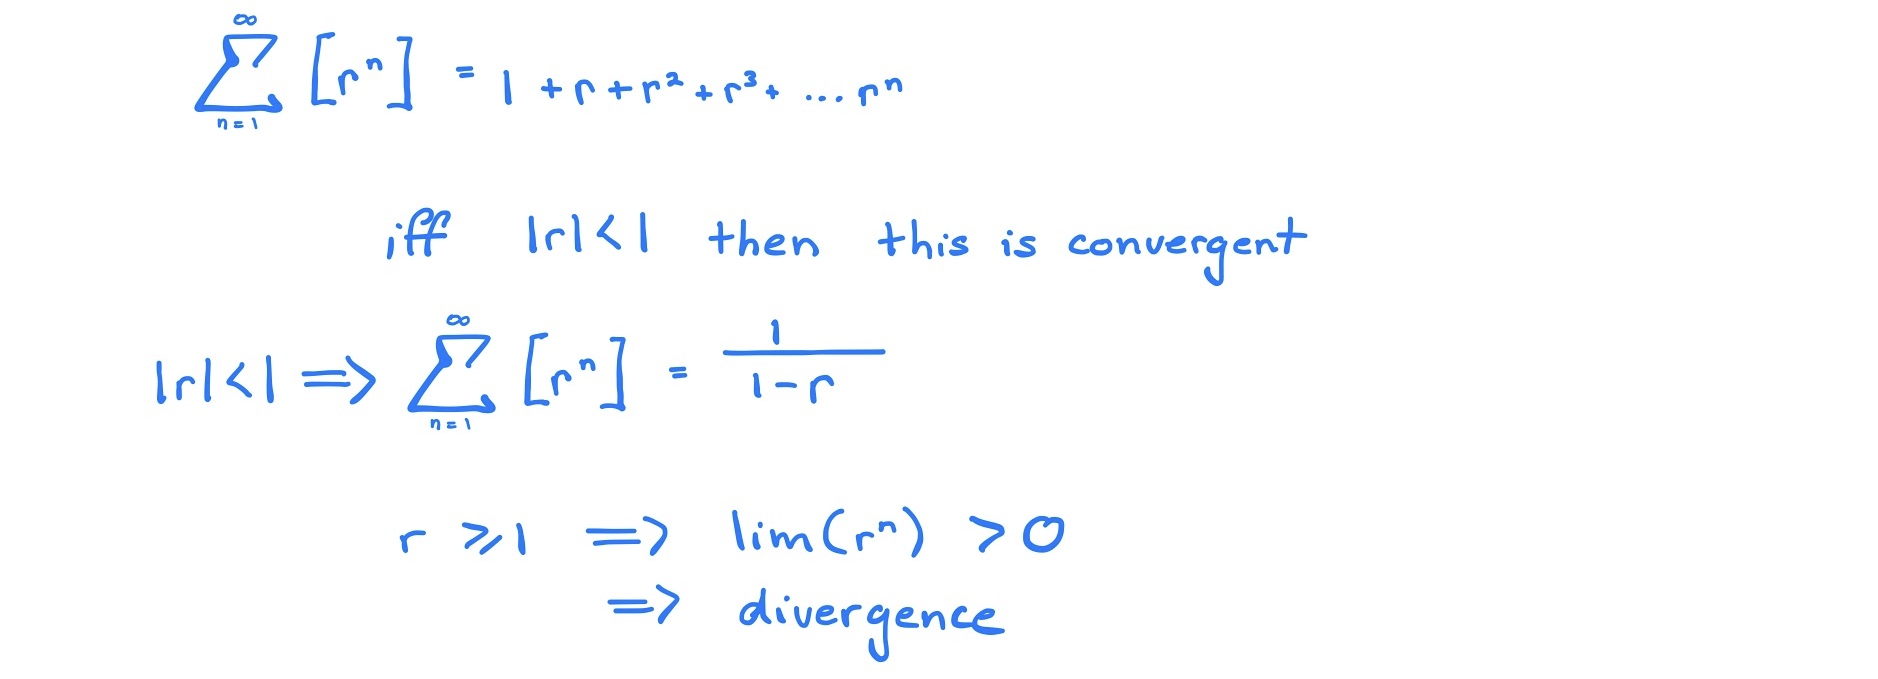
\includegraphics[width=5cm]{media/InfSeries/2B17FDDA-A24C-436F-B18E-73B69AF54A69.jpeg}
\caption{}
\end{figure}

\newpage
\hypertarget{header-n3155}{%
\subsubsection{Harmonic Series (3.7.6(b))}\label{header-n3155}}

\begin{figure}
\centering
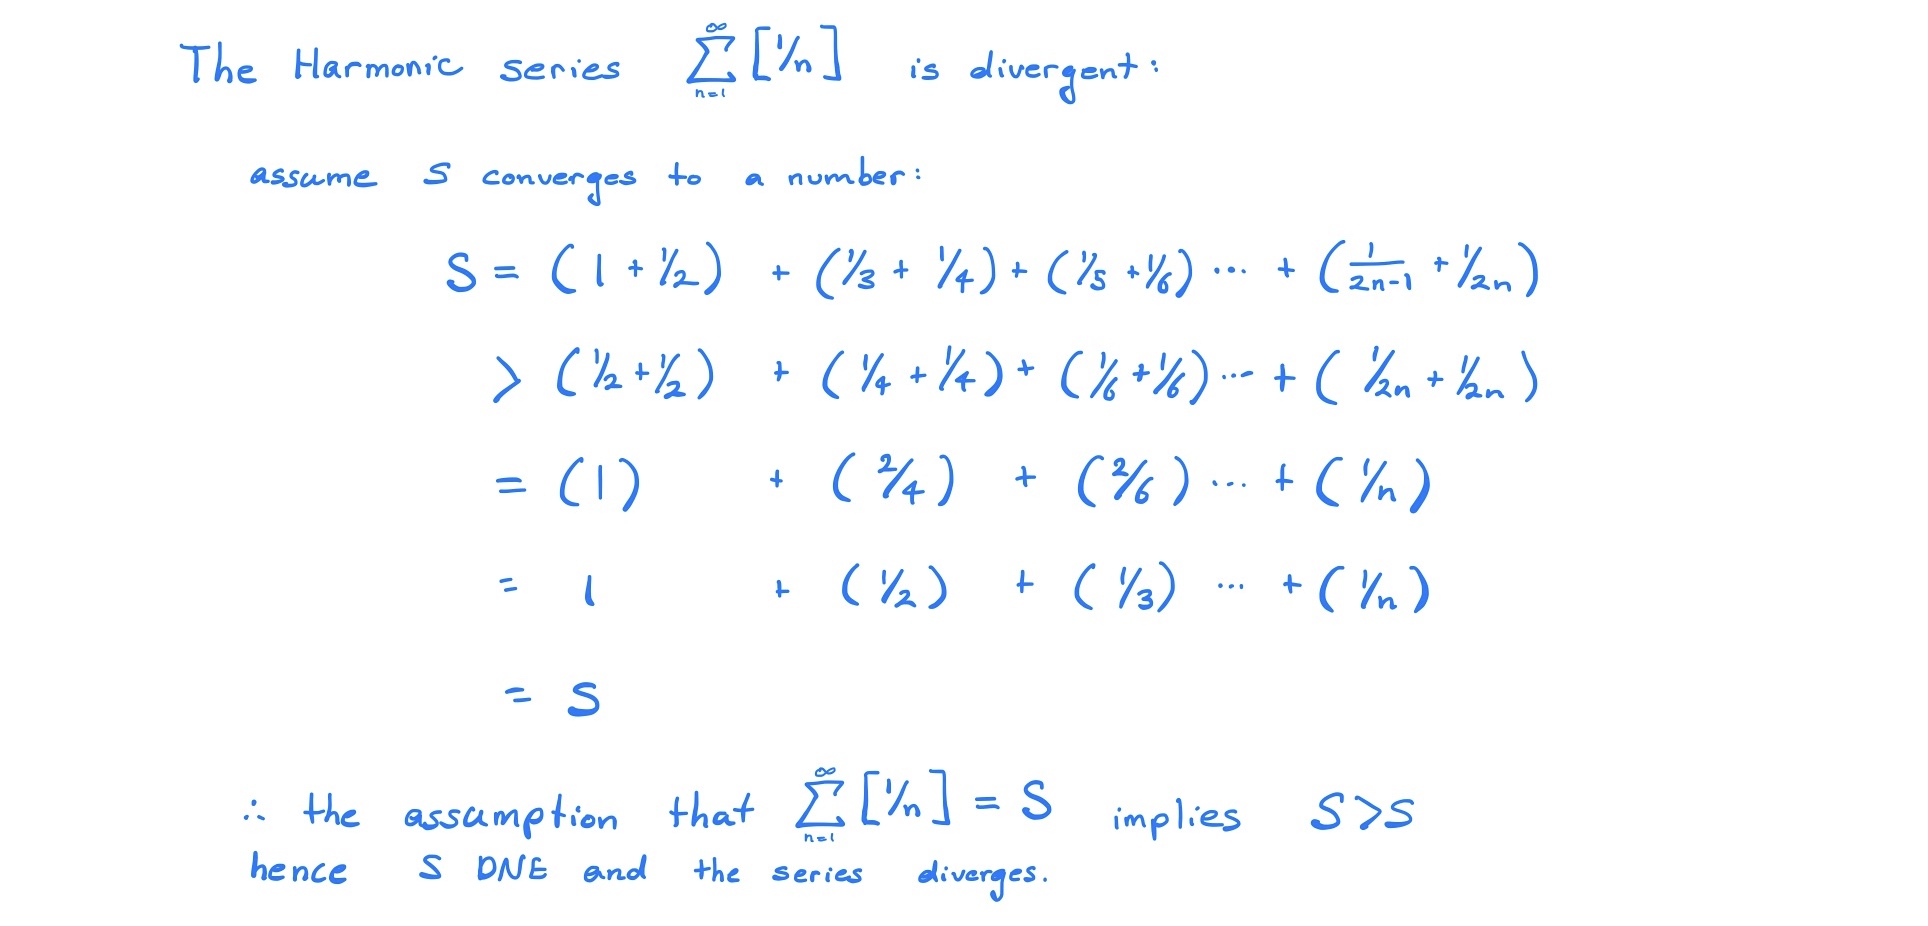
\includegraphics[width=5cm]{media/InfSeries/404880AA-8097-4857-B8DB-25933E988C53.jpeg}
\caption{}
\end{figure}

\hypertarget{header-n3157}{%
\subsubsection{\texorpdfstring{\(P\)-Series}{P-Series}}\label{header-n3157}}

\begin{figure}
\centering
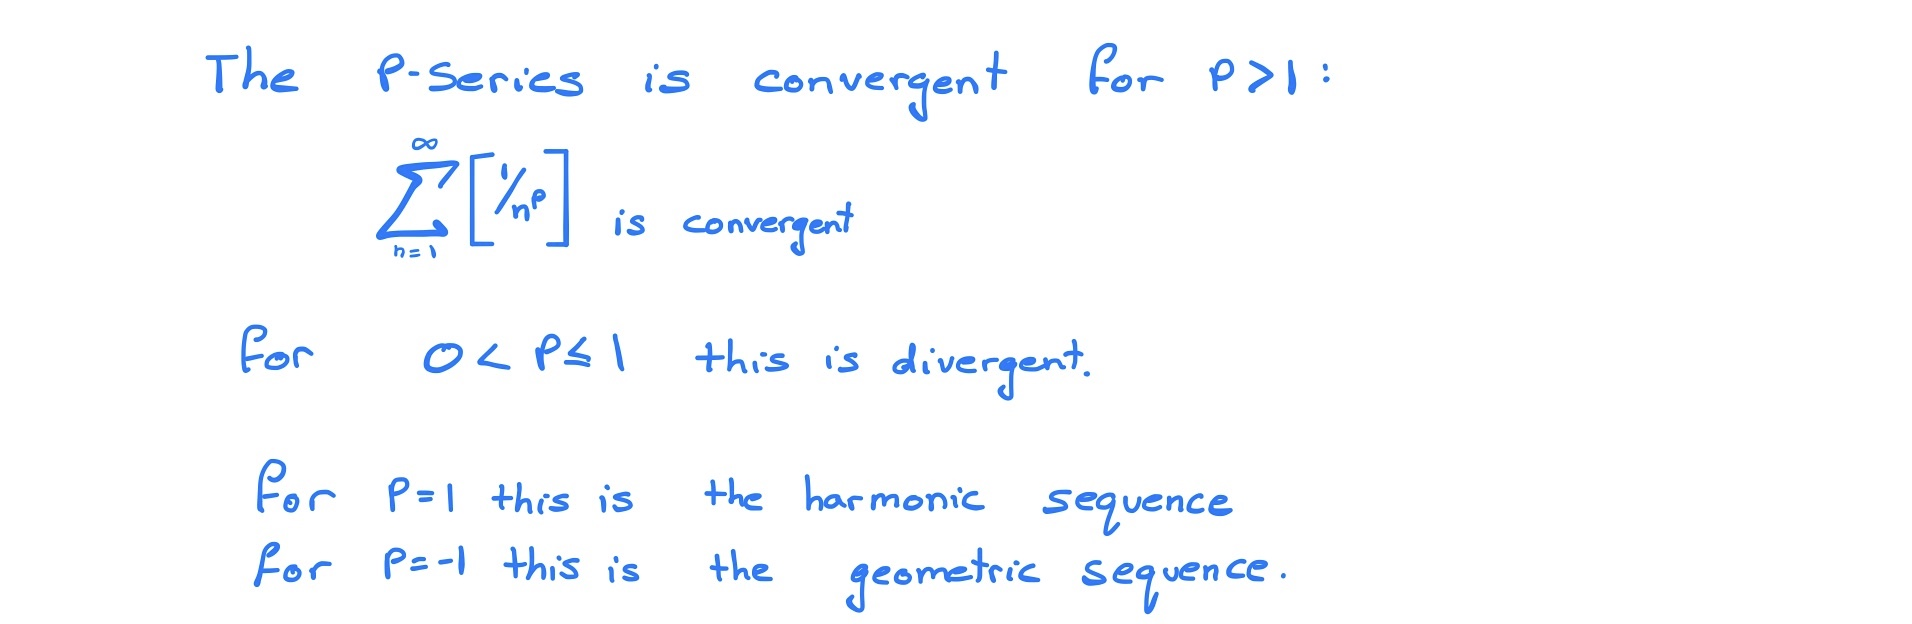
\includegraphics[width=5cm]{media/InfSeries/69F206AD-EF00-417C-95ED-31DAD675B9A5.jpeg}
\caption{}
\end{figure}

\newpage
\hypertarget{header-n3160}{%
\subsection{Properties of Series}\label{header-n3160}}

\hypertarget{header-n3161}{%
\subsubsection{\texorpdfstring{The \(n^\text{th}\) term
test}{The n\^{}\textbackslash text\{th\} term test}}\label{header-n3161}}

This is more or less a test for divergence, it is necessary that a
sequence \((x_n)\) has a limit of 0 in order for the series to be
convergent:

\[\exists L : \quad \sum_{n=1}^\infty \left[ x_n \right] = L \implies \lim(x_n)=0\]

be careful however because a sequence with a limit of 0 is not
sufficient to establish the convergence of a series:

\[\exists L : \quad \sum_{n=1}^\infty \left[ x_n \right] = L \nRightarrow \lim(x_n)=0\]

\hypertarget{header-n3167}{%
\subsubsection{Cauchy Criterion for series}\label{header-n3167}}

If a sequence is convergent it must be a Cauchy sequence, hence all
convergent series are composed of \emph{Cauchy Sequences} (as a
necessary but not sufficient condition).

So to be clear a series converges if and only if it is a \emph{Cauchy
Sequence}.

\hypertarget{header-n3170}{%
\subsubsection{Definitions}\label{header-n3170}}

\begin{itemize}
\item
  A Cauchy Sequence is:

  \begin{itemize}
  \item
    \(\forall \varepsilon > 0, \exists M : \enspace m,n \geq M \implies \mid s_m -s_n \mid = \left| x_{n+1} + x_{n+2} + x_{n+3} \dots x_m \right| < \varepsilon\)
  \end{itemize}
\item
  A Series Converges (which is an equivalent statement) if:

  \begin{itemize}
  \item
    \(\forall \varepsilon > 0, \exists M : \enspace ,n \geq N \implies \mid s_n -s \mid = \left| x_{1} + x_{2} + x_{3} \dots x_n \right| < \varepsilon\)
  \end{itemize}
\end{itemize}


\newpage
\hypertarget{header-n3182}{%
\subsection{Convergence Tests}\label{header-n3182}}

\hypertarget{header-n3183}{%
\subsubsection{Types of Convergence}\label{header-n3183}}

A series \(\sum [x_n]\) is \textbf{\emph{absolutely convergent}} if and
only if \(\sum \left[  \enspace \left| x_n \right| \enspace \right]\) ,
otherwise the series is said to be conditionally convergent.

This is important because
\(\textsf{the convergence of } \sum \left[  \enspace \left| x_n \right| \enspace \right] \implies \textsf{the convergence of} \sum [x_n]\)

Below the tests have been split into three categories:

\begin{itemize}
\item
  Comparison Tests

  \begin{itemize}
  \item
    These establish non-absolute convergence but are broadly applicable
    and so are introduced early
  \end{itemize}
\item
  Absolute Convergence Tests

  \begin{itemize}
  \item
    These establish absolute convergence.
  \end{itemize}
\item
  Non-Absolute Convergence Tests

  \begin{itemize}
  \item
    These are useful for \emph{alternating Series} and series that
    change sign as they progress (e.g. \(\frac{sin(n)}{n}\))
  \end{itemize}
\end{itemize}

\hypertarget{header-n3203}{%
\subsubsection{Choosing a Test}\label{header-n3203}}

Choosing the right test can be difficult, hence I have included an
appendix with a
\href{http://tutorial.math.lamar.edu/Classes/CalcII/SeriesStrategy.aspx}{flow
chart} \footnote{Strategy for Series,
  http://tutorial.math.lamar.edu/Classes/CalcII/SeriesStrategy.aspx}
that we should probably memorise for want of the exam



\hypertarget{header-n3206}{%
\subsubsection{Manipulating Series}\label{header-n3206}}

Sometimes you'll be given a series in an odd way for example:

\[S_n = \sum^\infty_{n=1} \left[ \frac{1}{(3n-2)\cdot (3n+1)} \right]\]

Now this could be shown to be convergent using the limit comparison test
(which is below) but if you are asked to find the value to which the
series converges to there is a bit more work involved.

Generally if you are asked to find what value a series converges to it
will be either:

\begin{itemize}
\item
  A Geometric Series (3.7.6(a) of TB), or
\item
  A telescoping Series
\end{itemize}

Geometric Series have already been shown, but a telescoping series is
new and not covered in the textbook, basically, it is a series where
most of the terms cancel out by way of rearrangement and grouping to
leave only one or two terms left.



\hypertarget{header-n3218}{%
\paragraph{Partial Fractions}\label{header-n3218}}

Often it is necessary to manipulate the terms somewhat in order for them
to exhibit the cancelling/telescoping property, often by way of partial
fractions (remember from \emph{Mathematics1B}), for an example of this
refer to Q3(c) of the corresponding tutorial
\(\tiny \textsf{(tutorial \#4 of wk 4 material, due wk. 5, topic 3 from learning guide)}\)

In this case because the provided series is not a geometric series it
must be a telescoping series (because otherwise we wouldn't be asked to
find the value to which it converges to, we only know how to find the
convergence values of those two series, so we know it's telescoping, in
order to get it into a form that will work, use partial fractions
\footnote{Partial Fractions,
  \href{Pauls\%20Calculus}{http://tutorial.math.lamar.edu/Classes/CalcII/PartialFractions.aspx}}

\begin{figure}
\centering
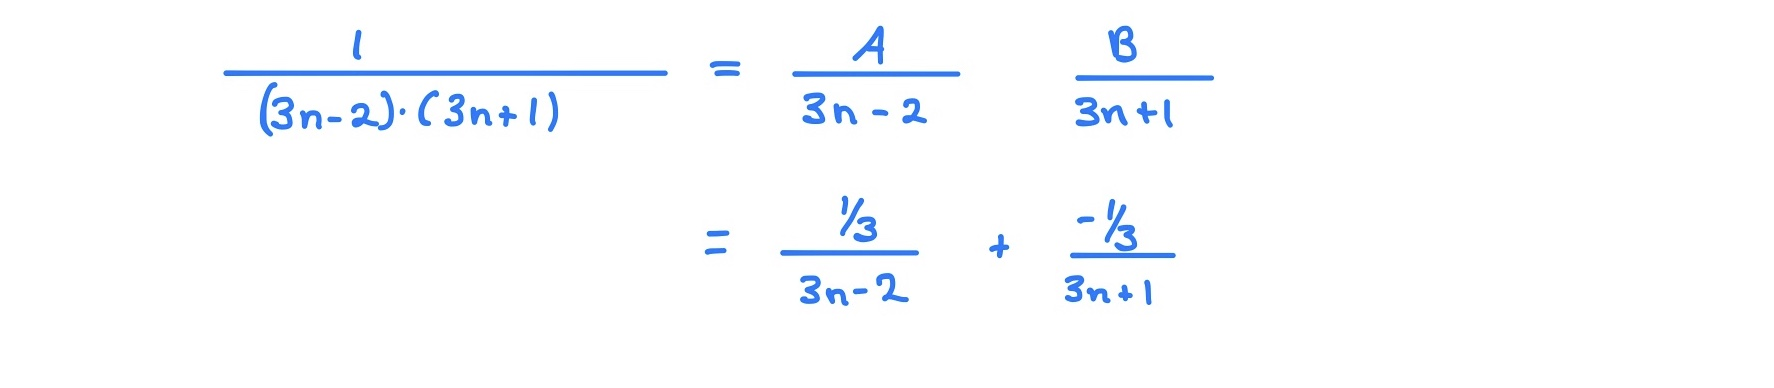
\includegraphics[width=5cm]{media/InfSeries/55CCA5D8-0B0A-438D-A991-6DB931F19D72.jpeg}
\caption{}
\end{figure}

From here we would manipulate the series using grouping and
rearrangement

\hypertarget{header-n3223}{%
\paragraph{Grouping Series}\label{header-n3223}}

Grouping terms in a series does not affect the value to which it
converges,

\begin{itemize}
\item
  This flows from the associativity of addition, a property exhibited by
  the \(\mathbb{R}\) which is the codomain of the sequence function
\end{itemize}

So in the above example the regrouping necessary to demonstrate the
telescoping nature:

\begin{figure}
\centering
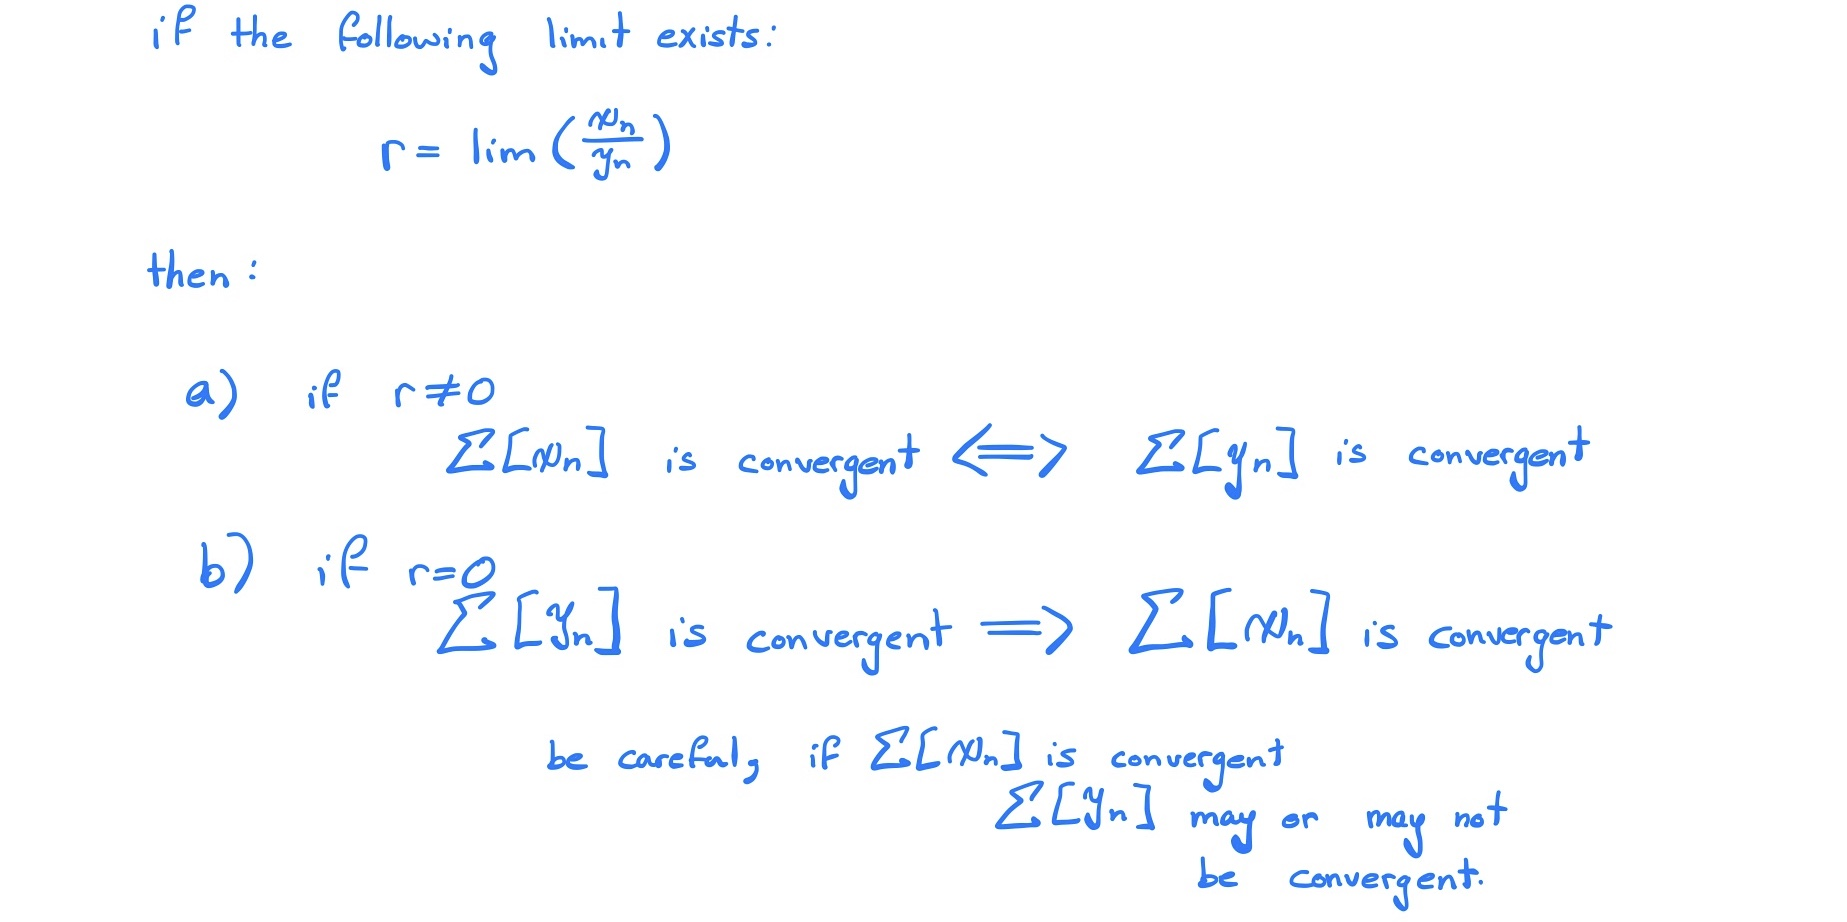
\includegraphics[width=5cm]{media/InfSeries/67331FF8-C7AD-4BE3-ADAE-2D291C4A5D89.jpeg}
\caption{}
\end{figure}

\newpage
\hypertarget{header-n3232}{%
\paragraph{Rearrangements (9.1.5)}\label{header-n3232}}

If a series is absolutely convergent then you can rearrange the terms
and the series will converge to the same value (otherwise you can't so
be careful)

\begin{itemize}
\item
  So say you have some series and you rearrange it, if this new series
  is absolutely convergent thet it's fine.
\item
  However, if you rearrange some series and the new series is only
  conditionally convergent, then the rearrangement wasn't logically
  valid and this convergence value is erroneous. 
\end{itemize}

So in our example the series is absolutely convergent so we could
rearrange it:

\begin{figure}
\centering
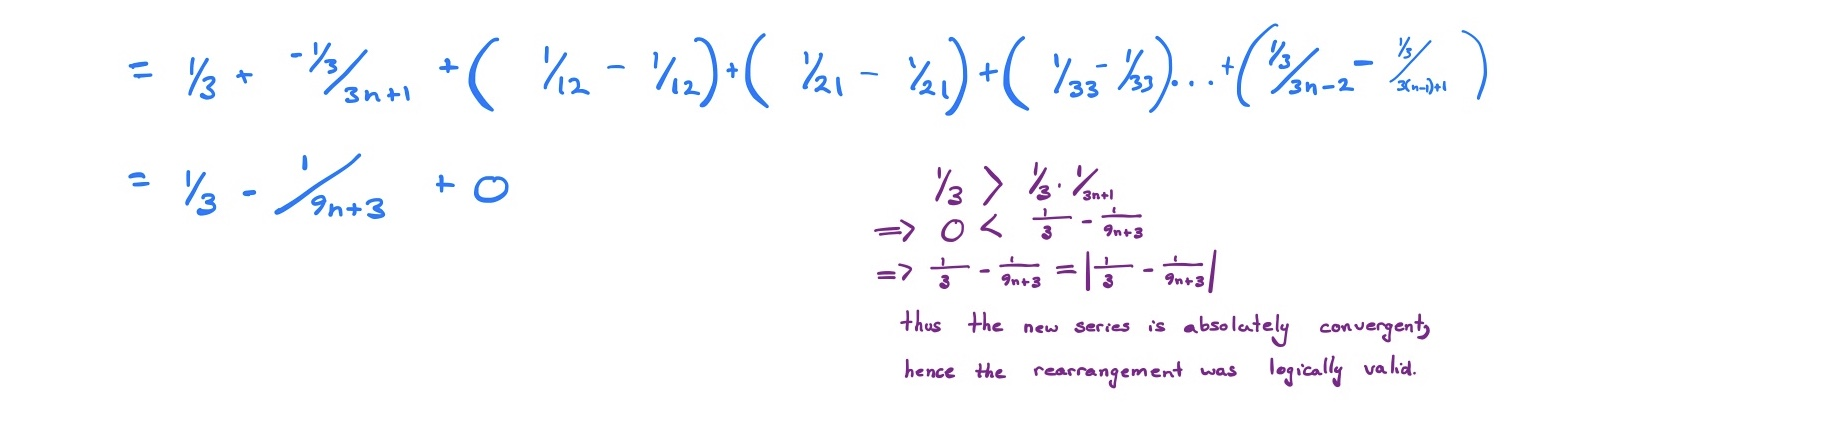
\includegraphics[width=5cm]{media/InfSeries/83FE5712-DC18-44D6-A9A3-FF7CB63F6AE9.jpeg}
\caption{}
\end{figure}

\newpage
\hypertarget{header-n3241}{%
\subsubsection{Identities to remember}\label{header-n3241}}

For the exam We need to remember these identities:

\hypertarget{header-n3243}{%
\paragraph{\texorpdfstring{Limit of
\(e^\frac{1}{n}\)}{Limit of e\^{}\textbackslash frac\{1\}\{n\}}}\label{header-n3243}}

\begin{figure}
\centering
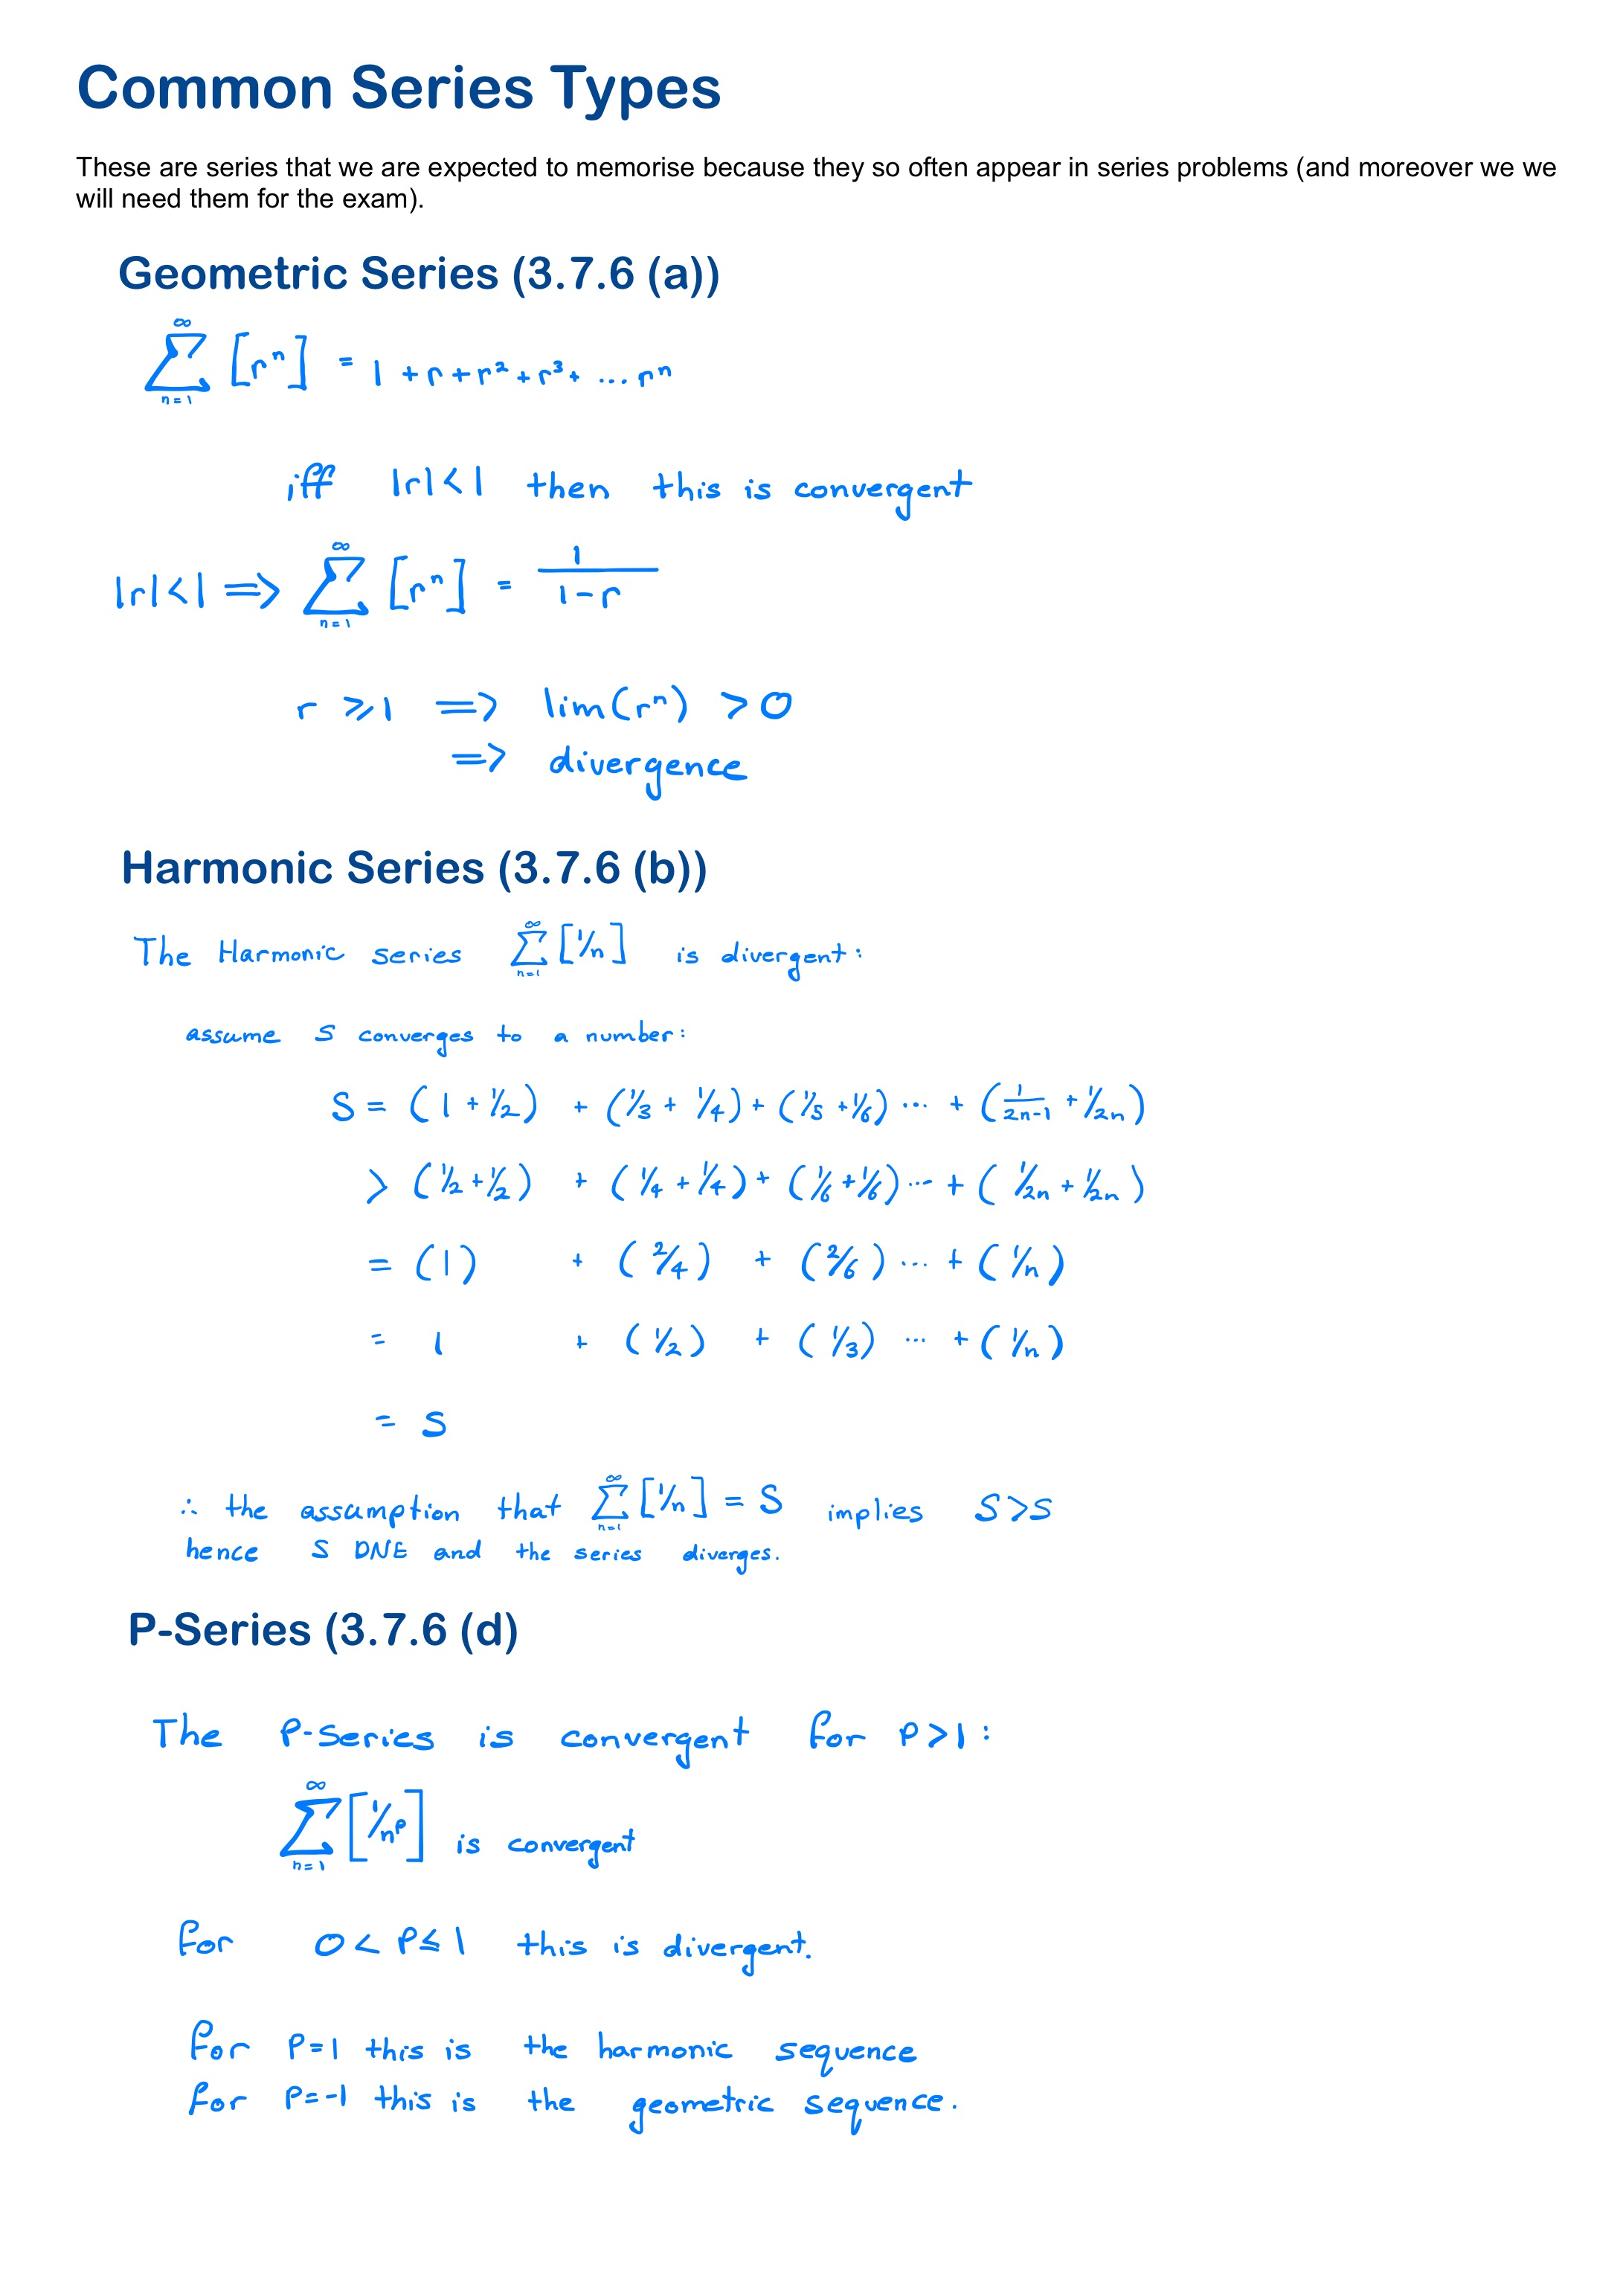
\includegraphics[width=5cm]{media/InfSeries/5E521A99-BC9F-40B8-8FE7-4B35EB40DC43.jpeg}
\caption{}
\end{figure}

\hypertarget{header-n3245}{%
\paragraph{Dealing with Inequalities}\label{header-n3245}}

\begin{figure}
\centering
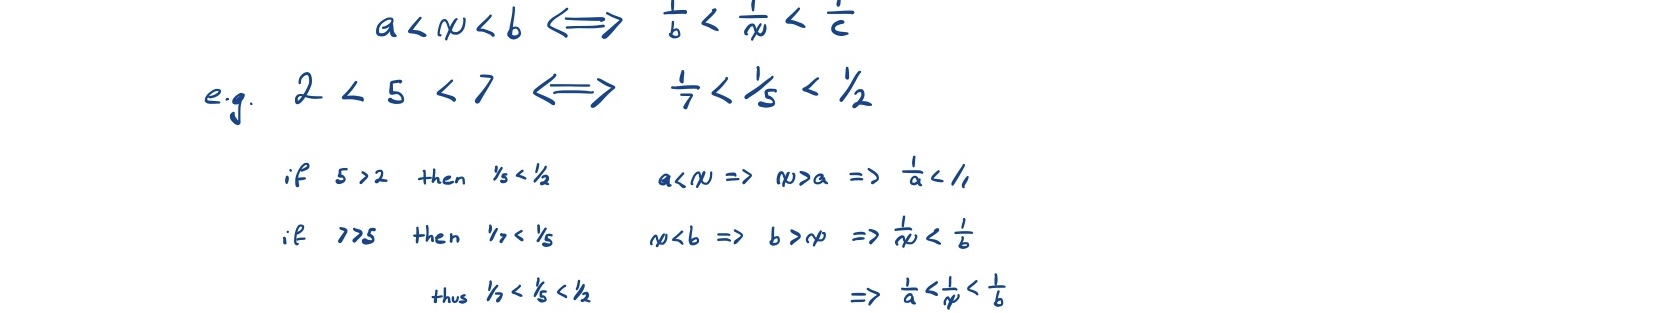
\includegraphics[width=5cm]{media/InfSeries/C613EA1A-E507-4DED-8B75-9A7B87BA17C1.jpeg}
\caption{}
\end{figure}

\newpage

\hypertarget{header-n3247}{%
\subsubsection{Comparison Tests}\label{header-n3247}}

\hypertarget{header-n3248}{%
\paragraph{Comparison Test (3.7.7)}\label{header-n3248}}

\begin{figure}
\centering
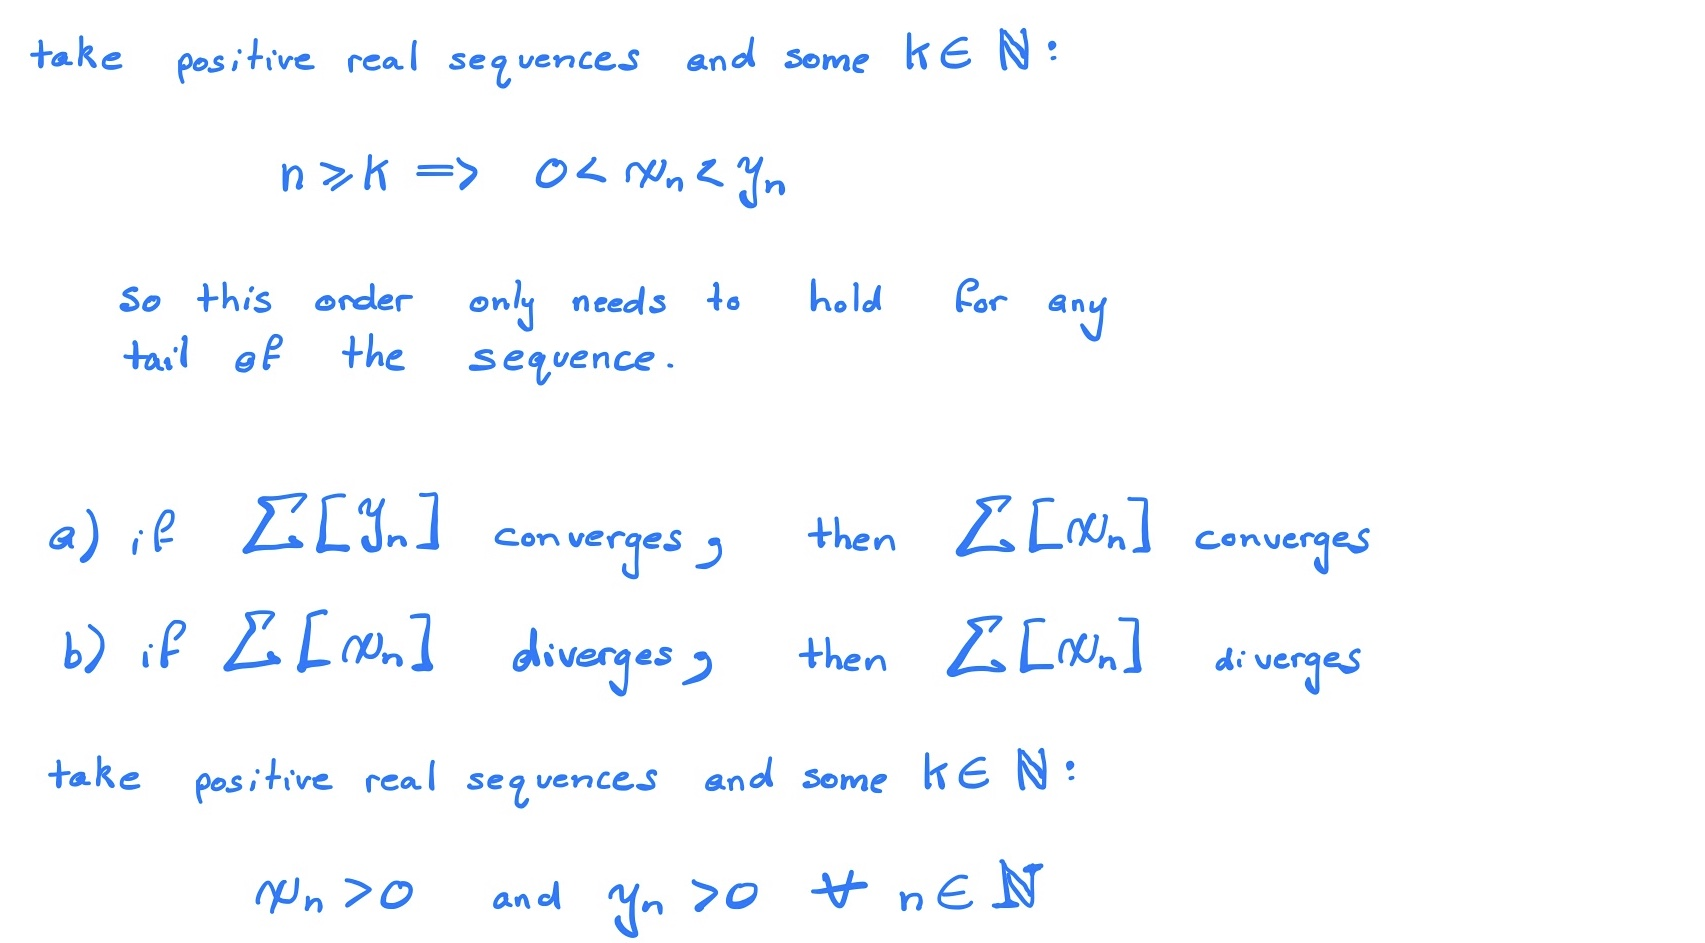
\includegraphics[width=5cm]{media/InfSeries/FD08303A-128F-49B5-80ED-4EBD48B1A48F.jpeg}
\caption{}
\end{figure}

\hypertarget{header-n3250}{%
\paragraph{Limit Comparison Test (3.7.8)}\label{header-n3250}}

Sometimes it can be difficult to establish the inequealities of the
first test and a ratio would be easier to use, in that case this test
can be used:
\ \\
\ \\
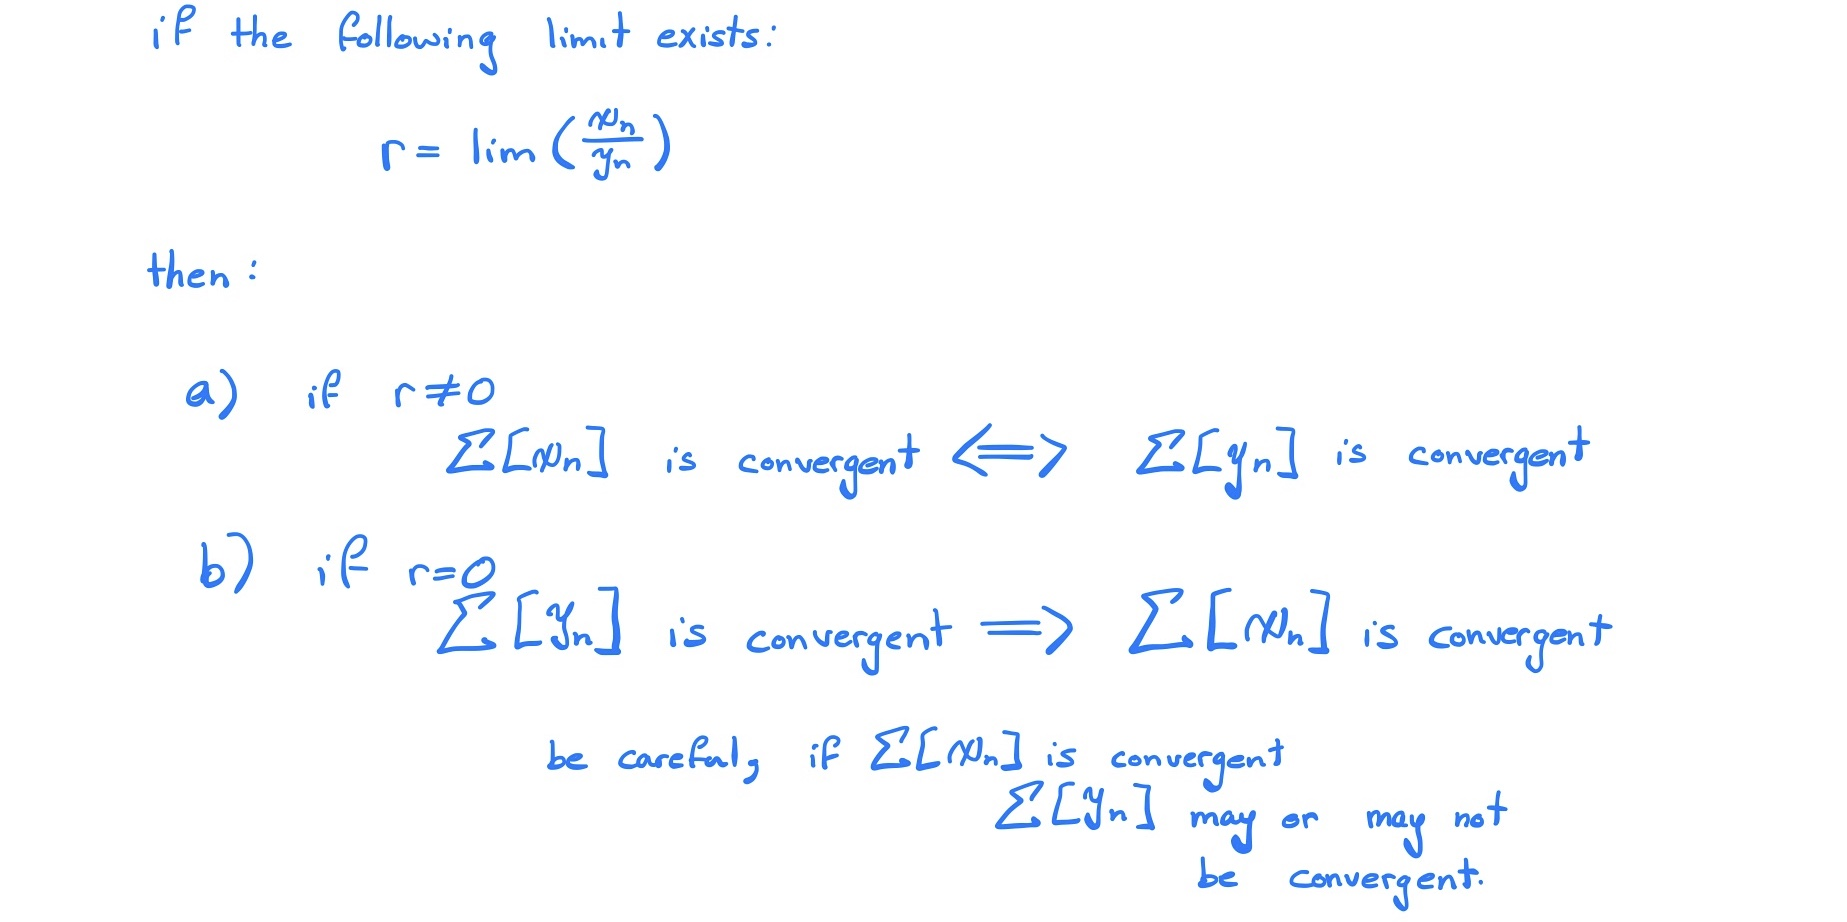
\includegraphics[width=5cm]{media/InfSeries/67331FF8-C7AD-4BE3-ADAE-2D291C4A5D89.jpeg}

\hypertarget{header-n3253}{%
\subsubsection{Absolute Convergence Tests}\label{header-n3253}}

If these tests are satisfied they will establish that the series is
absolutely convergent.

\hypertarget{header-n3255}{%
\paragraph{Limit Comparison Test II (9.2.1) (For Absolute
Convergence)}\label{header-n3255}}

This version of the test is useful for establishing absolute
convergence, it may be more difficult to establish however.

\begin{figure}
\centering
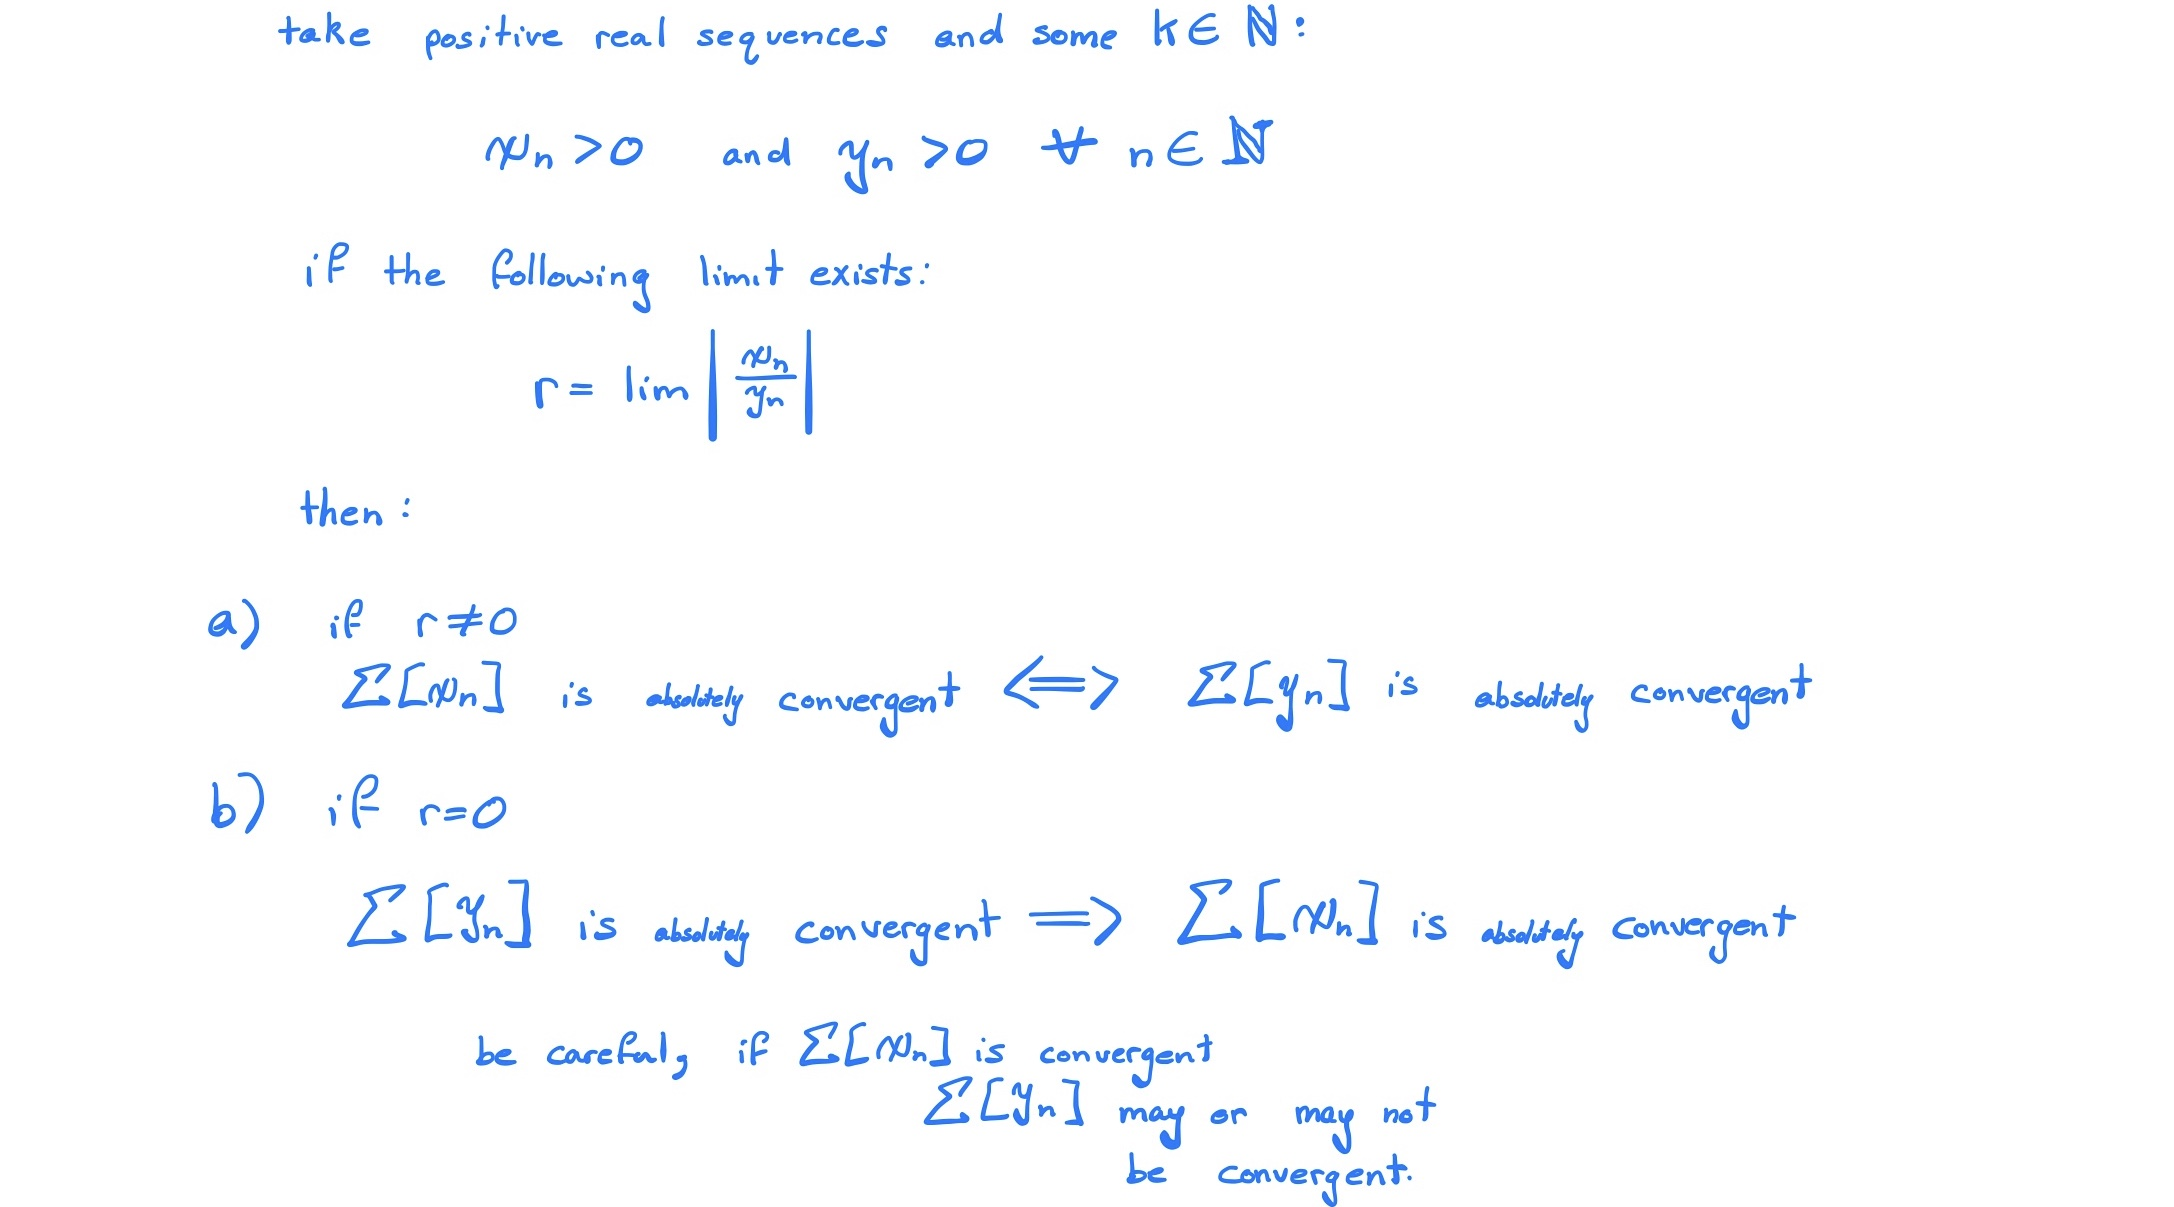
\includegraphics[width=5cm]{media/InfSeries/DEEDB59D-00EA-4BF3-A5F9-7571412B11C2.jpeg}
\caption{}
\end{figure}

\newpage
\hypertarget{header-n3259}{%
\paragraph{Ratio Test (9.2.4)}\label{header-n3259}}

\hypertarget{header-n3261}{%
\subparagraph{Generalised D'Alambert}\label{header-n3261}}

This can be useful where the ratio test fails for want of \((-1)^{n+1}\)
because the \(\limsup()\) operator will strip that way for a \((+1)\).

It is worth remembering that a sequence \((x_n)\) is convergent if and
only if:

\[\liminf(x_n) = \limsup(x_n)=\lim(x_n)\]

In this test however, we simply need to show that the \(\limsup\) exists
(which it will if the ratio-sequence has an upper bound), it isn't
necessary to show that the ratio-sequence is convergent.

\begin{itemize}
\item
  (However, it is necessary that the sequence which generates the series
  converges to 0, otherwise the series will be divergent)
\end{itemize}

\newpage 

\hypertarget{header-n3270}{%
\paragraph{Root Test}\label{header-n3270}}

\begin{figure}
\centering
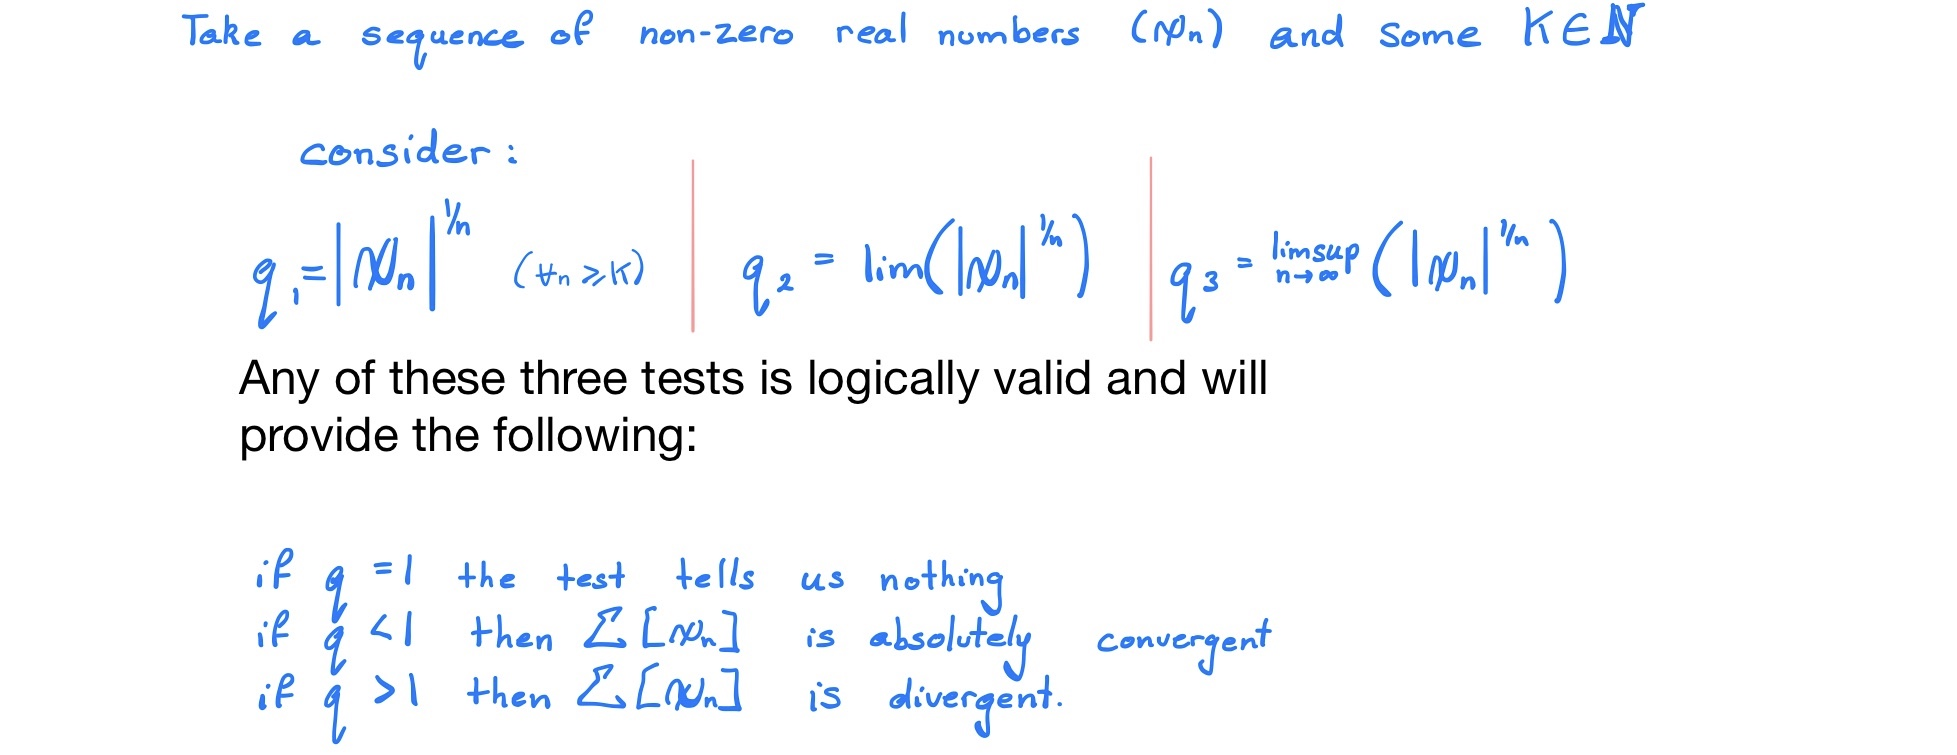
\includegraphics[width=5cm]{media/InfSeries/8D469008-5118-4138-808A-3A9480B23FA5.jpeg}
\caption{}
\end{figure}

\hypertarget{header-n3274}{%
\subparagraph{\texorpdfstring{Generalised \emph{Cauchy}
Test}{Generalised Cauchy Test}}\label{header-n3274}}

This can be useful where the root test fails for want of \((-1)^n\), the
\(\limsup()\) operator will strip that away for a \((+1)\).

\hypertarget{header-n3276}{%
\paragraph{Integral Test}\label{header-n3276}}

If the series is of a function that is positive and ecreasint, then the
series could converge if and only if the integral converges:

Let \(f(k)\) be a positive decreasing function and let \(k\) be some
natural number:

\[\exists L\in \mathbb{R} : \enspace L = \sum^\infty_{n=k} \left[ f(k) \right] \ \iff \int_\infty^k \! f(x) \, \mathrm{d}x = \lim_{b\rightarrow\infty}\left( \int_b^k \! f(x) \, \mathrm{d}x\right)\]

Or basically the series will converge if and only if the corresponding
integral converges,

\begin{itemize}
\item
  This flows from the notion that the area under a continuous curve is
  going to be greater than the various term values, hence by the
  comparison test it's going to converge.
\item
  this is a test for absolute convergence because the terms of the
  sequence that generates the series are strictly positive as a
  prerequisite anyway.
\end{itemize}

\newpage 

\hypertarget{header-n3286}{%
\subsubsection{Non-Absolute Convergence Tests}\label{header-n3286}}

\hypertarget{header-n3287}{%
\paragraph{Definition of an Alternating Sequence
(9.3.1)}\label{header-n3287}}

An alternating sequence is a sequence that changes sign at each
iteration, so for example \((x_n) = \frac{(-1)^{n+1}}{n}\) is an
alternating sequence because at each succession the sequence changes
sign \((x_n) = \frac{\sin(n}{n}\) is not an alternating sequence because
the terms doesn't alternate at each succession:

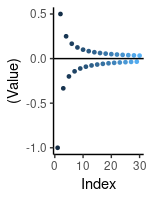
\includegraphics[width=5cm]{media/InfSeries/Rplot.png}
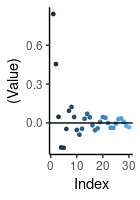
\includegraphics[width=5cm]{media/InfSeries/Rplot01.png}

\hypertarget{header-n3292}{%
\paragraph{Alternating Series Test}\label{header-n3292}}

Take a decreasing sequence of positive numbers \((Z_n)\), :

\begin{itemize}
\item
  If the sequence is such that:

  \begin{itemize}
  \item
    \(Z_{n+1} < Z_n \enspace  \enspace \wedge \enspace Z_n > 0 \qquad \forall n \in \mathbb{n}\)
  \end{itemize}
\item
  Then the series will be convergent:

  \begin{itemize}
  \item
    \(\exists L \in \mathbb(R): \enspace \sum^\infty_{n=1} \left[ (-1)^{n+1} \cdot Z_n \right]\)
  \end{itemize}
\end{itemize}

So basically if the sequence is decreasing, then the series of the
alternating sequence will hence converge.

\hypertarget{header-n3307}{%
	\newpage
\paragraph{Partial Summation Formula (Abel's
Lemma)}\label{header-n3307}}

Let \(X: = \left( x_n \right)\) and \(Y:= \left( y_n \right)\) by
sequences in \(\mathbb{R}\) and let the partial sums of
\(\sum\left( y_n \right)\) be denoted by \(\left( s_)n \right)\) with
\(s_0 : = 0\)

\[\sum_{k=n+1}^{m}\left[ x_ky_k \right]=\left( x_ms_m - x_{n+1}s_n \right) + \sum{k=n+1}^{m-1}\left( x_k-x_k+1 \right)s_k
  \label{partsum}\]



\hypertarget{header-n3311}{%
\paragraph{Dirichlet's Test}\label{header-n3311}}

\begin{figure}
\centering
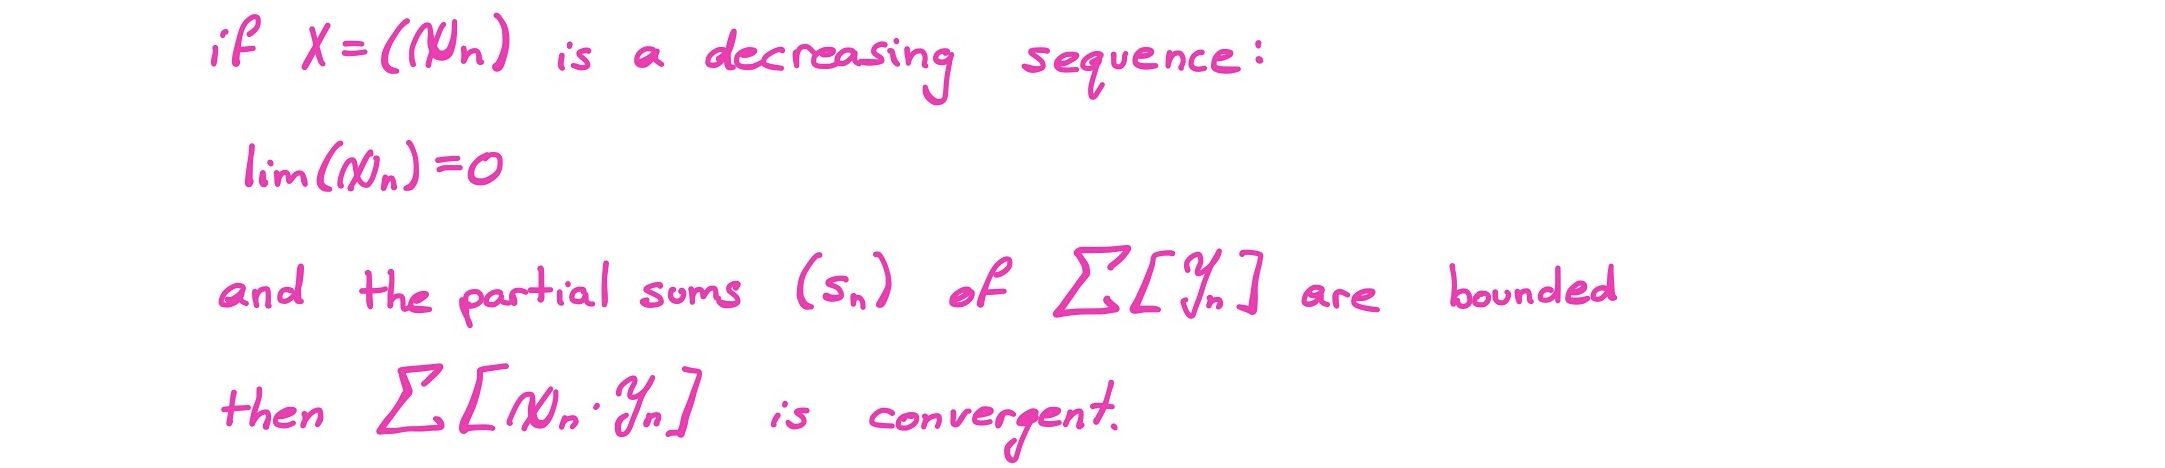
\includegraphics[width=5cm]{media/InfSeries/BE23258A-CC18-49A6-AABB-E71063CAF34C.jpeg}
\caption{}
\end{figure}

\hypertarget{header-n3314}{%
\paragraph{Abel's Test}\label{header-n3314}}

\begin{figure}
\centering
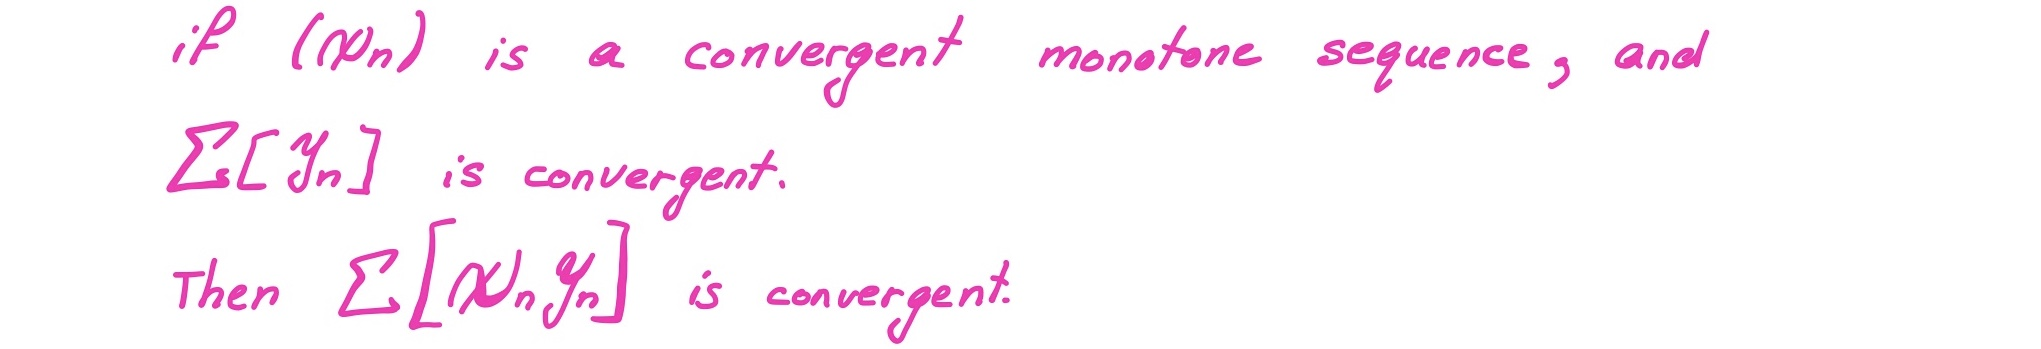
\includegraphics[width=5cm]{media/InfSeries/6360D524-9307-4308-94C1-BCA6D2E0ECE7.jpeg}
\caption{}
\end{figure}

\end{document}
